%!TEX root = ./main.tex
%
% This file is part of the i10 thesis template developed and used by the
% Media Computing Group at RWTH Aachen University.
% The current version of this template can be obtained at
% <https://hci.rwth-aachen.de/karrer_thesistemplate>.

\chapter{Programmkonzeption}

In diesem Abschnitt gehe ich auf die Konzeptionelle Phase des Programms näher. Dabei beschreibe ich die Programmstruktur mittels UML-Klassendiagramme. Mit einer Sequenzdiagramm ist das Programmablauf gut veranschaulicht worden. Schließlich folgt eine genauere Beschreibung der verwendeten Methoden mittels Nassi-Schneiderman-Diagrammen.

\section{Klassen}
Das Programm beinhaltet folgende Klassen:

\subsection{\texttt{Main}}
    
    Die Hauptklasse für das Programm T9.
    Diese Klasse beinhaltet die Einsprungfunktion des gesamten Programms. Es Wird ein Wörterbuch sowie eine Konsole erstellt. die Konsole wird gestartet und nach Ende der Nutzerinteraktion wieder beendet.
    
\subsection{\texttt{Konsole}}
    
    Diese Klasse ist die Konsole für die Nutzerinteraktion. Beim Starten der Konsole wird das Wörterbuch aus einer Datei geladen. Bei diesem Vorgang wird der Nutzer benachrichtigt, ob das Wörterbuch geladen ist oder nicht.
    Die Konsole verwaltet die Eingaben und Ausgaben des Programms. Die Eingaben vom Nutzer werden gefiltert und nach Richtigkeit geprüft. Im Falle einer Falschen Eingabe, wird ein Fehler auf der Konsole mit folgender Form gezeigt:\newline
    Falsche Eingabe\newline
    \textless Grund\textgreater
    \newline
    Mögliche Ausgaben:
    \begin{enumerate}
        \item Kein Woerterbuch geladen
        \item Woerterbuch geladn
        \item Kein passendes Wort gespeichert. Eingabe im Explizitmodus:
        \item \textless Wort-Vorschlag\textgreater
        \item Wort ok?
        \item Wort gespeichert
        \item Der Satz lautet \textless gebildeter Satz\textgreater
        \item Programmende.
    \end{enumerate}{}
    Alle Ausgaben mit den \textless \textgreater -Klammern sind dynamisch.
    
    
    
\subsection{\texttt{Woerterbuch}}
    
    Diese Klasse repräsentiert das Wörterbuch des Programms T9. Die Klasse beinhaltet eine Tabelle in Form einer HashMap, um die Speicherung des Wörterbuchs sowie das Lesen aus einer Textdatei zu vereinfachen.
    Die Klasse beinhaltet einen \textit{Baum} für die Textsuche, eine integer Zahl als festgelegte Größe des Wörterbuches und eine Pfadangabe als String für die Textdatei des Wörterbuchs.
    Die Methode \texttt{ladeBib} lädt das Wörterbuch aus der Textdatei. Dabei wird bei Fehler keine Datei geladen.
    Die Methode \texttt{speichereBib} speichert das Woerterbuch in der Textdatei. Bei Fehler wird nicht gespeichert und keine Fehlermeldung zurückgegeben.
    Für die Suche sowie Hinzufügen eines Wortes wird in der Klasse \texttt{Baum} die Suchfunktion sowie die \texttt{add}-Funktion aufgerufen. \texttt{add} fügt ein Wort sowohl im HashMap als auch im Baum.
    Beim Erstellen eines Baumes wird die Methode \texttt{makeTree} aufgerufen, die ein Baum für die vereinfachte Suche erstellt. Dabei werden alle Einträge im HashMap gelesen und im Baum gespeichert.
    Die Verwandlung von einer expliziten Ziffernfolge in einem Wort im Alphabet übernimmt die statische Methode \texttt{makeWord}. Diese Methode wird auch in der Klasse \texttt{Baum} verwendet, um gesuchte Ziffernfolgen umzuwandeln.
    
\subsection{\texttt{Baum}}
    
    Beinhaltet alle Einträge des Wörterbuchs im Form von Baumstruktur. Alle Knoten sind von der Klasse \texttt{Node}.
    Der Wurzelknoten ist eine ArrayList \textbf{root}, die alle Knoten enthält. \texttt{search} bekommt ein \textbf{key}, ein String von Ziffernfolge, und sucht rekursiv nach einem Treffer im Baum. Falls kein Treffer gefunden ist wird der String -1 zurückgegben. Um Wörter aus einem Endknoten zu konstruieren, wird \texttt{constructWord} mit einem Knoten aufgerufen. Diese Methode sucht alle Elternknoten der Reihe nach und speichert die Indexen der Knoten in einem String. Der String wird rückwärts umgewandelt und zu einem Wort mit Hilfe von \texttt{makeWord} interpretiert. Um ein Wort im Baum hinzufügen wird \texttt{add} aufgerufen. Diese Methode Wird rekursiv aufgerufen um Knoten im Baum hinzufügen oder falls schon vorhanden aktualisieren. Die Methode bekommt also eine explizite Ziffernfolge und ein Häufigkeit des Wortes. Falls keine Häufigkeit von einem Wort existiert wird die Methode 0 bekommen. Falls die Häufigkeit 0 ist, wird jedesmal, wenn ein bereits im Baum gespeichertes Wort erneut ausgewählt wird, wird seine Häufigkeit um eins erhöht.
    
\subsection{\texttt{Node}}
    
    Die Klasse repräsentiert einen Knoten im \texttt{Baum}. Sie beinhaltet Integerzahl n als Häufigkeit sowie ein Integerzahl als Index, ArrayList aus Node für allen Kindknoten und ein Node für einen Elternknoten.
    Die Methode \texttt{has} prüft nach Existenz eines Kindknotens und die Methode \texttt{get} liefert einer der Kindknoten mit einem eingegebenen Index.


\clearpage

\section{UML-Klassendiagramm}
%
%\begin{figure}[!ht]
%\centering
%\includegraphics[width=\textwidth]{../../src/resources/uml.png}
%\caption[UML-Klassendiagramm]{UML-Klassendiagramm der implementierten Klassen}
%\end{figure}

\section{Aktivitätsdiagramm zum Programmablauf}
Eine detaillierte Beschreibung des Programmablaufs anhand eines Aktivitätsdiagramm. Dies verdeutlich den Lebenszyklus mit den Kontroll-Beziehungen.
\begin{figure}[H]
\centering
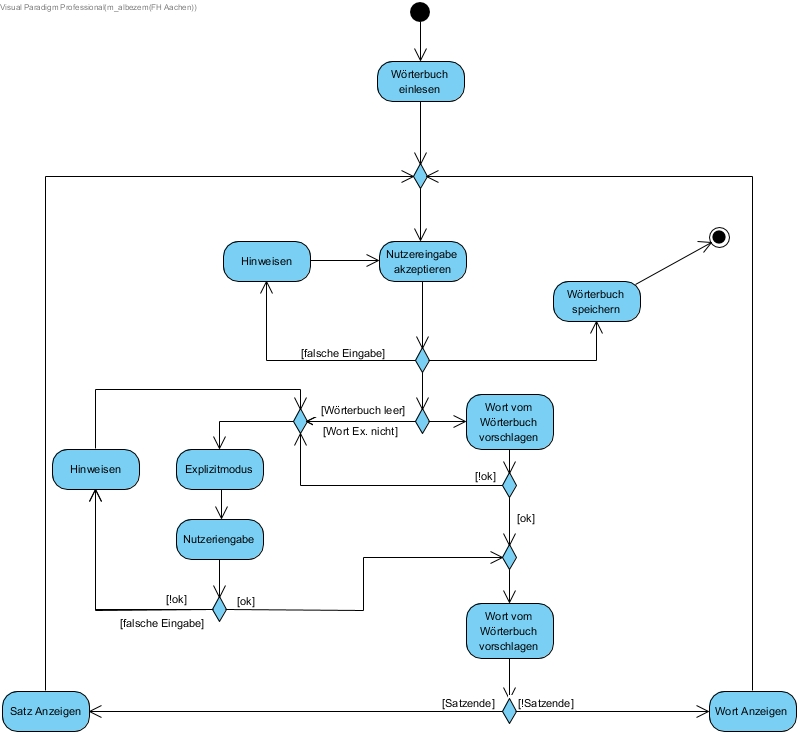
\includegraphics[width=1.\columnwidth]{images/activitydiagramm.jpg}
\caption[UML-Sequenzdiagramm]{UML-Aktivitätsdiagramm zum Programmablauf}
\end{figure}

\section{Beschreibung der Methoden}
Eine detailierte Beschreibung der Methoden folgt in Form von Nassi-Schneiderman-Diagrammen bzw. Struktogrammen.

\begin{figure}[!ht]
\centering
\includegraphics[width=\textwidth]{../../src/resources/toUpper.png}
\caption[UML-Klassendiagramm]{Algorithmus zur Umwandlung von Buchstaben in einem String zu Großbuchstaben}
\end{figure}

\begin{figure}[!ht]
\centering
\includegraphics[width=\textwidth]{../../src/resources/readInputFile.png}
\caption[UML-Klassendiagramm]{Algorithmus zum Lesen von Input-Datei}
\end{figure}
